% Options for packages loaded elsewhere
\PassOptionsToPackage{unicode}{hyperref}
\PassOptionsToPackage{hyphens}{url}
\PassOptionsToPackage{dvipsnames,svgnames,x11names}{xcolor}
%
\documentclass[
]{book}
\title{BFW Equilibrium Gender LFP and Wage Code Companion}
\author{Sonia R. Bhalotra, Manuel Fernández, and Fan Wang}
\date{2022-02-12}

\usepackage{amsmath,amssymb}
\usepackage{lmodern}
\usepackage{iftex}
\ifPDFTeX
  \usepackage[T1]{fontenc}
  \usepackage[utf8]{inputenc}
  \usepackage{textcomp} % provide euro and other symbols
\else % if luatex or xetex
  \usepackage{unicode-math}
  \defaultfontfeatures{Scale=MatchLowercase}
  \defaultfontfeatures[\rmfamily]{Ligatures=TeX,Scale=1}
\fi
% Use upquote if available, for straight quotes in verbatim environments
\IfFileExists{upquote.sty}{\usepackage{upquote}}{}
\IfFileExists{microtype.sty}{% use microtype if available
  \usepackage[]{microtype}
  \UseMicrotypeSet[protrusion]{basicmath} % disable protrusion for tt fonts
}{}
\makeatletter
\@ifundefined{KOMAClassName}{% if non-KOMA class
  \IfFileExists{parskip.sty}{%
    \usepackage{parskip}
  }{% else
    \setlength{\parindent}{0pt}
    \setlength{\parskip}{6pt plus 2pt minus 1pt}}
}{% if KOMA class
  \KOMAoptions{parskip=half}}
\makeatother
\usepackage{xcolor}
\IfFileExists{xurl.sty}{\usepackage{xurl}}{} % add URL line breaks if available
\IfFileExists{bookmark.sty}{\usepackage{bookmark}}{\usepackage{hyperref}}
\hypersetup{
  pdftitle={BFW Equilibrium Gender LFP and Wage Code Companion},
  pdfauthor={Sonia R. Bhalotra, Manuel Fernández, and Fan Wang},
  colorlinks=true,
  linkcolor={Maroon},
  filecolor={Maroon},
  citecolor={Blue},
  urlcolor={blue},
  pdfcreator={LaTeX via pandoc}}
\urlstyle{same} % disable monospaced font for URLs
\usepackage{longtable,booktabs,array}
\usepackage{calc} % for calculating minipage widths
% Correct order of tables after \paragraph or \subparagraph
\usepackage{etoolbox}
\makeatletter
\patchcmd\longtable{\par}{\if@noskipsec\mbox{}\fi\par}{}{}
\makeatother
% Allow footnotes in longtable head/foot
\IfFileExists{footnotehyper.sty}{\usepackage{footnotehyper}}{\usepackage{footnote}}
\makesavenoteenv{longtable}
\usepackage{graphicx}
\makeatletter
\def\maxwidth{\ifdim\Gin@nat@width>\linewidth\linewidth\else\Gin@nat@width\fi}
\def\maxheight{\ifdim\Gin@nat@height>\textheight\textheight\else\Gin@nat@height\fi}
\makeatother
% Scale images if necessary, so that they will not overflow the page
% margins by default, and it is still possible to overwrite the defaults
% using explicit options in \includegraphics[width, height, ...]{}
\setkeys{Gin}{width=\maxwidth,height=\maxheight,keepaspectratio}
% Set default figure placement to htbp
\makeatletter
\def\fps@figure{htbp}
\makeatother
\setlength{\emergencystretch}{3em} % prevent overfull lines
\providecommand{\tightlist}{%
  \setlength{\itemsep}{0pt}\setlength{\parskip}{0pt}}
\setcounter{secnumdepth}{5}
\usepackage{bbm}
\usepackage{booktabs}
\usepackage{longtable}
\usepackage{array}
\usepackage{multirow}
\usepackage{wrapfig}
\usepackage{float}
% \floatplacement{figure}{H}
\usepackage[labelformat = empty]{caption}
\usepackage{colortbl}
\usepackage{pdflscape}
\usepackage{tabu}
\usepackage{threeparttable}
\usepackage{threeparttablex}
\usepackage[normalem]{ulem}
\usepackage{makecell}
\usepackage{xcolor}
\usepackage{geometry}
\geometry{
	a4paper,
	left=1.0in,
	right=1.0in,
	top=1.0in,
	bottom=1.0in,
}
\setcounter{secnumdepth}{5}
\setcounter{tocdepth}{5}
\ifLuaTeX
  \usepackage{selnolig}  % disable illegal ligatures
\fi
\usepackage[]{natbib}
\bibliographystyle{apalike}

\begin{document}
\maketitle

{
\hypersetup{linkcolor=}
\setcounter{tocdepth}{1}
\tableofcontents
}
\hypertarget{preface}{%
\chapter*{Preface}\label{preface}}
\addcontentsline{toc}{chapter}{Preface}

This is a work-in-progress Matlab package consisting of functions that solve the equilibrium gender labor force participation and wage model in \href{https://www.iza.org/person/2905/sonia-r-bhalotra}{Bhalotra}, \href{https://sites.google.com/view/manuelfernandezsierra}{Fernández} and \href{https://fanwangecon.github.io/}{Wang} (2022). Tested with \href{https://www.mathworks.com/products/matlab.html}{Matlab} 2021b \citep{matlab}.

All functions are parts of a matlab toolbox that can be installed:

\begin{quote}
Download and install the Matlab toolbox: \href{https://github.com/FanWangEcon/PrjLabEquiBFW/blob/master/PrjLabEquiBFW.mltbx}{PrjLabEquiBFW.mltbx}
\end{quote}

The Code Companion can also be accessed via the bookdown site and PDF linked below:

\begin{quote}
\href{https://fanwangecon.github.io/PrjLabEquiBFW/bookdown/BFW-Equilibrium-Gender-LFP-and-Wage-Code-Companion.pdf}{\textbf{bookdown pdf}}, \href{https://www.mathworks.com/matlabcentral/fileexchange/80164-PrjLabEquiBFW}{\textbf{MathWorks File Exchange}}
\end{quote}

This bookdown file is a collection of mlx based vignettes for functions that are available from \href{https://github.com/FanWangEcon/PrjLabEquiBFW}{PrjLabEquiBFW}. Each Vignette file contains various examples for invoking each function.

The package relies on \href{https://fanwangecon.github.io/MEconTools/}{MEconTools}, which needs to be installed first. The package does not include allocation functions, only simulation code to generate the value of each stimulus check increments for households.

The site is built using \href{https://bookdown.org/}{Bookdown} \citep{R-bookdown}.

Please contact \href{https://fanwangecon.github.io/}{FanWangEcon} for issues or problems.

\hypertarget{introduction}{%
\chapter{Introduction}\label{introduction}}

\hypertarget{bhalotra-fernuxe1ndez-and-wang-2022}{%
\section{Bhalotra, Fernández, and Wang (2022)}\label{bhalotra-fernuxe1ndez-and-wang-2022}}

In Bhalotra, Fernández, and Wang (2022).

\hypertarget{core-functions}{%
\chapter{Core Functions}\label{core-functions}}

\hypertarget{ces-demand-core-functions}{%
\section{CES Demand Core Functions}\label{ces-demand-core-functions}}

This is the example vignette for function:
\href{https://github.com/FanWangEcon/PrjLabEquiBFW/tree/main/PrjLabEquiBFW/func/bfw_mp_func_demand.m}{\textbf{bfw\_mp\_func\_demand}}
from the \href{https://fanwangecon.github.io/PrjLabEquiBFW/}{\textbf{PrjLabEquiBFW
Package}}\textbf{.} This
function generates a container map with key CES demand-side equation for
a particular sub-nest.

\hypertarget{default-test}{%
\subsection{Default Test}\label{default-test}}

Default test

\begin{verbatim}
bl_verbose = true;
mp_func_demand = bfw_mp_func_demand(bl_verbose);

----------------------------------------
xxxxxxxxxxxxxxxxxxxxxxxxxxxxxxxxxxxxxxxx
CONTAINER NAME: mp_func Functions
xxxxxxxxxxxxxxxxxxxxxxxxxxxxxxxxxxxxxxxx
                                i      idx                                                           functionString                                                      
                               ____    ____    __________________________________________________________________________________________________________________________

    fc_OMEGA                   "1"     "1"     "@(p1,p2,rho,beta_1,beta_2)p1.*fc_d1(p1,p2,1,1,rho,beta_1,beta_2)+p2.*fc_d2(p1,p2,1,1,rho,beta_1,beta_2)"                 
    fc_d1                      "2"     "2"     "@(p1,p2,Y,Z,rho,beta_1,beta_2)(Y/Z).*(beta_1+beta_2.*((p1./p2).*(beta_2./beta_1)).^(rho/(1-rho))).^(-1/rho)"             
    fc_d2                      "3"     "3"     "@(p1,p2,Y,Z,rho,beta_1,beta_2)(Y/Z).*(beta_1.*((p2./p1).*(beta_1./beta_2)).^(rho/(1-rho))+beta_2).^(-1/rho)"             
    fc_lagrange_x1             "4"     "4"     "@(p1,rho,beta_1,beta_2,x_1,x_2)p1/(((beta_1*x_1^(rho)+beta_2*x_2^(rho))^((1/rho)-1))*(beta_1*x_1^(rho-1)))"              
    fc_lagrange_x2             "5"     "5"     "@(p2,rho,beta_1,beta_2,x_1,x_2)p2/(((beta_1*x_1^(rho)+beta_2*x_2^(rho))^((1/rho)-1))*(beta_2*x_2^(rho-1)))"              
    fc_output_nest             "6"     "6"     "@(q1,q2,rho,beta_1,beta_2)((beta_1)*q1^(rho)+beta_2*q2^(rho))^(1/rho)"                                                   
    fc_p1_foc                  "7"     "7"     "@(lagrangem,rho,beta_1,beta_2,x_1,x_2)lagrangem*(((beta_1*x_1^(rho)+beta_2*x_2^(rho))^((1/rho)-1))*(beta_1*x_1^(rho-1)))"
    fc_p2_foc                  "8"     "8"     "@(lagrangem,rho,beta_1,beta_2,x_1,x_2)lagrangem*(((beta_1*x_1^(rho)+beta_2*x_2^(rho))^((1/rho)-1))*(beta_2*x_2^(rho-1)))"
    fc_share_given_elas_foc    "9"     "9"     "@(rho,p1,p2,x1,x2)fc_share_given_elas_foc_Q(rho,p1,p2,x1,x2)/(1+fc_share_given_elas_foc_Q(rho,p1,p2,x1,x2))"             
    fc_w1dw2                   "10"    "10"    "@(x_1,x_2,rho,beta_1,beta_2)(x_2/x_1)^(1-rho)*(beta_1/beta_2)"                                                           
    fc_yz_ratio                "11"    "11"    "@(p1,p2,q1,q2,rho,beta_1,beta_2)fc_revenue(p1,p2,q1,q2)/fc_OMEGA(p1,p2,rho,beta_1,beta_2)"                               
\end{verbatim}

\hypertarget{demand}{%
\chapter{Demand}\label{demand}}

\hypertarget{solving-nested-ces-demand-problems-crs}{%
\section{Solving Nested CES Demand Problems (CRS)}\label{solving-nested-ces-demand-problems-crs}}

Taking advantage of
\href{https://github.com/FanWangEcon/PrjLabEquiBFW/blob/main/PrjLabEquiBFW/solvedemand/bfw_crs_nested_ces.m}{\textbf{bfw\_crs\_nested\_ces}}
from the \href{https://fanwangecon.github.io/PrjLabEquiBFW/}{\textbf{PrjLabEquiBFW
Package}}\textbf{.} This
function solves optimal choices in Constant Elasticity of Substitution
problems with constant returns and two inputs in each sub-nest. Takes as
inputs share and elasticity parameters across layers of sub-nests, as
well as input unit costs at the bottom-most layer. Works for CES
problems with up to four nest layers, and allows for uneven branches, so
that some branches go up to four layers, but others have less layers.
Works with BFW (2022) nested labor input problem.

\hypertarget{key-inputs-and-outputs-for-bfw_mp_func_demand}{%
\subsection{\texorpdfstring{Key Inputs and Outputs for \href{https://github.com/FanWangEcon/PrjLabEquiBFW/tree/main/PrjLabEquiBFW/func/bfw_mp_func_demand.m}{\textbf{bfw\_mp\_func\_demand}}}{Key Inputs and Outputs for bfw\_mp\_func\_demand}}\label{key-inputs-and-outputs-for-bfw_mp_func_demand}}

Here are the key inputs for the CES demand solver function:

\begin{itemize}
\item
  \textbf{FL\_YZ} float output divided by productivity, aggregate single
  term
\item
  \textbf{CL\_MN\_PRHO} cell array of rho (elasticity) parameter between
  negative infinity and 1. For example, suppose there are four nest
  layers, and there are two branches at each layer, then we have 1, 2,
  4, and 8 \(\rho\) parameter values at the 1st, 2nd, 3rd, and 4th nest
  layers: size(CL\_MN\_PRHO\{1\})= \(\left\lbrack 1,1\right\rbrack\),
  size(CL\_MN\_PRHO\{2\}) = \(\left\lbrack 1,2\right\rbrack\),
  size(CL\_MN\_PRHO\{3\}) = \(\left\lbrack 2,2\right\rbrack\),
  size(CL\_MN\_PRHO\{4\}) = \(\left\lbrack 2,2,2\right\rbrack\). Note that
  if the model has 4 nest layers, not all cells need to be specified,
  some branches could be deeper than others.
\item
  \textbf{CL\_MN\_PSHARE} cell array of share (between 0 and 1) for the first
  input of the two inputs for each nest. The structure for this is
  similar to CL\_MN\_PRHO.
\item
  \textbf{CL\_MN\_PRICE} cell array of wages for both wages for the first and
  second nest, the last index in each element of the cell array
  indicates first (1) or second (2) wage. For example, suppose we have
  four layers, with 2 branches at each layer, as in the example for
  CL\_MN\_PRHO, then we have 2, 4, 8, and 16 wage values at the 1st,
  2nd, 3rd, and 4th nest layers: size(CL\_MN\_PRICE\{1\}) =
  \(\left\lbrack 1,2\right\rbrack\), size(CL\_MN\_PRICE\{2\}) =
  \(\left\lbrack 2,2\right\rbrack\), size(CL\_MN\_PRICE\{3\}) =
  \(\left\lbrack 2,2,2\right\rbrack\), size(CL\_MN\_PRICE\{4\}) =
  \(\left\lbrack 2,2,2,2\right\rbrack\) . Note that only the last layer
  of wage needs to be specified, in this case, the 16 wages at the 4th
  layer. Given optimal solutions, we solve for the 2, 4, and 8
  aggregate wages at the higher nest layers. If some branches are
  deeper than other branches, then can specific NA for non-reached
  layers along some branches.
\item
  \textbf{BL\_BFW\_MODEL} boolean true by default if true then will output
  outcomes specific to the BFW 2022 problem.
\end{itemize}

Here are the key outputs for the CES demand solver function:

\begin{itemize}
\item
  \textbf{CL\_MN\_YZ\_CHOICES} has the same dimension as CL\_MN\_PRICE, suppose
  there are four layers, the CL\_MN\_PRICE\{4\} results at the lowest
  layer includes quantity choices that might be observed in the data.
  CL\_MN\_PRICE cell values at non-bottom layers include aggregate
  quantity outcomes.
\item
  \textbf{CL\_MN\_PRICE} includes at the lowest layer observed wages,
  however, also includes higher layer aggregate solved waves.
  CL\_MN\_PRHO and CL\_MN\_PSHARE are identical to inputs.
\end{itemize}

\hypertarget{single-nest-layer-two-inputs-ces-problem}{%
\subsection{Single Nest Layer Two Inputs CES Problem}\label{single-nest-layer-two-inputs-ces-problem}}

In this first example, we solve a constant returns to scale problem with
a single nest, meaning just two inputs and a single output.

\begin{verbatim}
clc;
close all;
clear all;

% Output requirement
fl_yz = 1;
% rho = 0.5, 1/(1-0.5)=2, elasticity of substitution of 2
cl_mn_prho = {[0.1]};
% equal share, similar "productivity"
cl_mn_pshare = {[0.5]};
% wages for the two inputs, identical wage
cl_mn_price = {[1, 1]};
% print option
bl_verbose = true;
mp_func = bfw_mp_func_demand();
bl_bfw_model = false;
[cl_mn_yz_choices, cl_mn_price, cl_mn_prho, cl_mn_pshare] = ...
    bfw_crs_nested_ces(fl_yz, cl_mn_prho, cl_mn_pshare, cl_mn_price, ...
    mp_func, bl_verbose, bl_bfw_model);

----------------------------------------
xxxxxxxxxxxxxxxxxxxxxxxxxxxxxxxxxxxxxxxx
CONTAINER NAME: mp_container_map ND Array (Matrix etc)
xxxxxxxxxxxxxxxxxxxxxxxxxxxxxxxxxxxxxxxx
                i    idx    ndim    numel    rowN    colN    sum    mean    std    coefvari    min    max
                _    ___    ____    _____    ____    ____    ___    ____    ___    ________    ___    ___

    price_c1    1     2      2        2       1       2       2      1       0        0         1      1 
    yz_c1       2     4      2        2       1       2       2      1       0        0         1      1 

xxx TABLE:price_c1 xxxxxxxxxxxxxxxxxx
          c1    c2
          __    __

    r1    1     1 

xxx TABLE:yz_c1 xxxxxxxxxxxxxxxxxx
          c1    c2
          __    __

    r1    1     1 

----------------------------------------
xxxxxxxxxxxxxxxxxxxxxxxxxxxxxxxxxxxxxxxx
CONTAINER NAME: mp_container_map Scalars
xxxxxxxxxxxxxxxxxxxxxxxxxxxxxxxxxxxxxxxx
                 i    idx    value
                 _    ___    _____

    prho_c1      1     1      0.1 
    pshare_c1    2     3      0.5 
\end{verbatim}

\hypertarget{single-nest-layer-two-inputs-ces-problem-vary-share-and-elasticity}{%
\subsection{Single Nest Layer Two Inputs CES Problem, Vary Share and Elasticity}\label{single-nest-layer-two-inputs-ces-problem-vary-share-and-elasticity}}

In this second example, we test over different rho values, explore
optimal relative choices, as share and elasticity change. In this
exercise, we also check, at every combination of rho and share
parameter, whether the FOC condition is satisfied by the optimal
choices. Also check if at the optimal choices, the minimization output
requirement is met.

\begin{verbatim}
% Approximately close function
rel_tol=1e-09;
abs_tol=0.0;
if_is_close = @(a,b) (abs(a-b) <= max(rel_tol * max(abs(a), abs(b)), abs_tol));

% Define share and rho arrays
fl_yz = 1;
ar_pshare = linspace(0.1, 0.9, 9);
ar_prho = 1 - 10.^(linspace(-2, 2, 30));
% Loop over share and rho values
mt_rela_opti = NaN([length(ar_pshare), length(ar_prho)]);
mt_x1_opti = NaN([length(ar_pshare), length(ar_prho)]);
for it_pshare_ctr = 1:length(ar_pshare)
    for it_prho_ctr = 1:length(ar_prho)

        % A. Parameters
        % rho
        fl_prho = ar_prho(it_prho_ctr);
        cl_mn_prho = {[fl_prho]};
        % share
        fl_pshare = ar_pshare(it_pshare_ctr);
        cl_mn_pshare = {[fl_pshare]};
        % wages for the two inputs, identical wage
        cl_mn_price = {[1, 1]};
        % print option
        bl_verbose = false;

        % B. Call function
        [cl_mn_yz_choices, cl_mn_price, cl_mn_prho, cl_mn_pshare] = ...
            bfw_crs_nested_ces(fl_yz, cl_mn_prho, cl_mn_pshare, cl_mn_price, ...
            mp_func, bl_verbose, bl_bfw_model);
        % Store results for optimal choice
        fl_opti_x1 = cl_mn_yz_choices{1}(1);
        fl_opti_x2 = cl_mn_yz_choices{1}(2);
        mt_x1_opti(it_pshare_ctr, it_prho_ctr) = fl_opti_x1;

        % C. Check if relative optimality FOC condition is met
        fl_rela_opti = fl_opti_x1/fl_opti_x2;
        % From FOC give wages = 1 both
        % Using What is above Equation A.20 in draft.
        fl_rela_opti_foc = (((fl_pshare/(1-fl_pshare)))*(1))^(1/(1-ar_prho(it_prho_ctr)));
        if (~if_is_close(fl_rela_opti_foc, fl_rela_opti))
            error('There is an error, optimal relative not equal to expected foc ratio')
        end

        % D. Check if output quantity requirement is met
        fl_output = ((fl_pshare)*fl_opti_x1^(fl_prho) + (1-fl_pshare)*fl_opti_x2^(fl_prho))^(1/fl_prho);
        if (~if_is_close(fl_output, fl_yz))
            error('There is an error, output is not equal to required expenditure minimizing output')
        end

    end
end
\end{verbatim}

Key results: (1) As share of input 1 goes to zero, optimal choice goes
to zero when inputs are elastic; (2) When inputs are inelasticty, even
very low share input 1 asymptote to equal input 2; (3) When input 1 is
more productive (higher share), actually hire less as productivity
(share) increases, becasue less of it is needed to achieve production
for high rho, elastictic production function; (4) For inelastic
production, monotonic relationship between input and shares.

\begin{verbatim}
% Visualize
% Generate some Data
rng(456);
ar_row_grid = ar_pshare;
ar_col_grid = log(1-ar_prho)/log(10);
rng(123);
mt_value = mt_x1_opti;
% container map settings
mp_support_graph = containers.Map('KeyType', 'char', 'ValueType', 'any');
mp_support_graph('cl_st_graph_title') = {'Optimal input 1 choice, rho=x, share=color'};
mp_support_graph('cl_st_ytitle') = {'Optimal choice of input 1'};
mp_support_graph('cl_st_xtitle') = {'Rho in (1-log10(rho)) scale', ...
    'left = perfect substitution (rho = 1)', ...
    'right = perfect complements (negative infinity rho)'};
mp_support_graph('st_legend_loc') = 'southwest';
mp_support_graph('bl_graph_logy') = false; % do not log
mp_support_graph('st_rowvar_name') = 'share=';
mp_support_graph('it_legend_select') = 5; % how many shock legends to show
mp_support_graph('st_rounding') = '6.3f'; % format shock legend
mp_support_graph('cl_colors') = 'jet'; % any predefined matlab colormap
% Call function
ff_graph_grid(mt_value, ar_row_grid, ar_col_grid, mp_support_graph);
\end{verbatim}

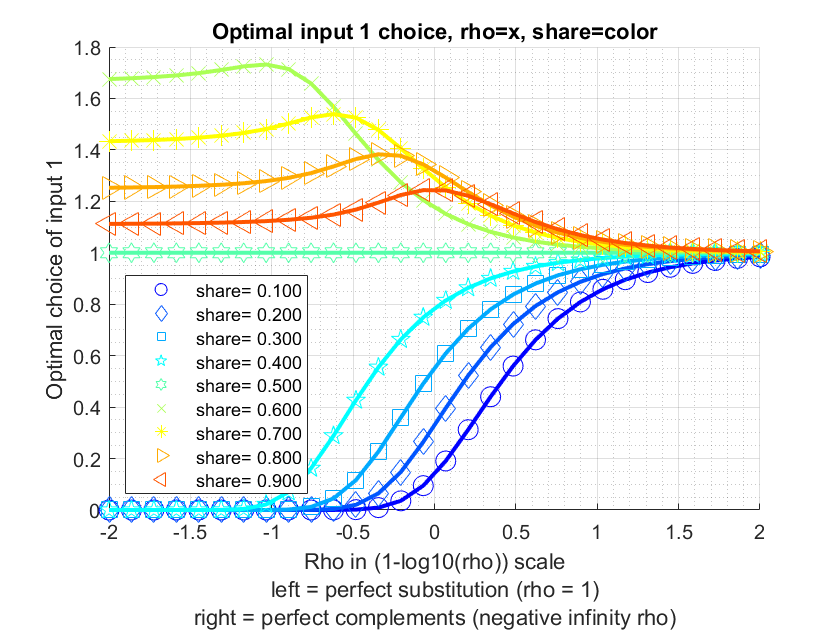
\includegraphics[width=5.20833in,height=\textheight]{img/bfwx_crs_nested_ces_images/figure_0.png}

\hypertarget{doubly-nest-layer-two-inputs-each-sub-nest-ces-problem}{%
\subsection{Doubly Nest Layer Two Inputs Each Sub-nest CES Problem}\label{doubly-nest-layer-two-inputs-each-sub-nest-ces-problem}}

In this third example, solve for optimal choices for a doubly nested
problem. Below, we first solve for the optimal choices, then we do a
number of checks, to make sure that the solutions are correct, as
expected.

\begin{verbatim}
% output requirement
fl_yz = 2.1;
% upper nest 0.1, lower nests 0.35 and -1 separately for rho values
cl_mn_prho = {[0.1], [0.35, -1]};
% unequal shares of share values
cl_mn_pshare = {[0.4], [0.3, 0.88]};
% differential wages
% in lower-left nest, not productive and very expensive, not very elastic
% last index for left or right,
cl_mn_price = {[nan, nan], [10, 1;3, 4]};
% print option
bl_verbose = true;
[cl_mn_yz_choices, cl_mn_price, cl_mn_prho, cl_mn_pshare] = ...
    bfw_crs_nested_ces(fl_yz, cl_mn_prho, cl_mn_pshare, cl_mn_price, ...
    mp_func, bl_verbose, bl_bfw_model);

----------------------------------------
xxxxxxxxxxxxxxxxxxxxxxxxxxxxxxxxxxxxxxxx
CONTAINER NAME: mp_container_map ND Array (Matrix etc)
xxxxxxxxxxxxxxxxxxxxxxxxxxxxxxxxxxxxxxxx
                 i    idx    ndim    numel    rowN    colN     sum       mean       std      coefvari      min        max  
                 _    ___    ____    _____    ____    ____    ______    ______    _______    ________    ________    ______

    prho_c2      1     2      2        2       1       2       -0.65    -0.325    0.95459    -2.9372           -1      0.35
    price_c1     2     3      2        2       1       2      7.7788    3.8894     2.0959    0.53886       2.4074    5.3714
    price_c2     3     4      2        4       2       2          18       4.5      3.873    0.86066            1        10
    pshare_c2    4     6      2        2       1       2        1.18      0.59    0.41012    0.69512          0.3      0.88
    yz_c1        5     7      2        2       1       2      4.4862    2.2431    0.68863      0.307       1.7561      2.73
    yz_c2        6     8      2        4       2       2      9.0506    2.2626     2.7086     1.1971     0.047893    6.0934

xxx TABLE:prho_c2 xxxxxxxxxxxxxxxxxx
           c1     c2
          ____    __

    r1    0.35    -1

xxx TABLE:price_c1 xxxxxxxxxxxxxxxxxx
            c1        c2  
          ______    ______

    r1    2.4074    5.3714

xxx TABLE:price_c2 xxxxxxxxxxxxxxxxxx
          c1    c2
          __    __

    r1    10    1 
    r2     3    4 

xxx TABLE:pshare_c2 xxxxxxxxxxxxxxxxxx
          c1      c2 
          ___    ____

    r1    0.3    0.88

xxx TABLE:yz_c1 xxxxxxxxxxxxxxxxxx
           c1       c2  
          ____    ______

    r1    2.73    1.7561

xxx TABLE:yz_c2 xxxxxxxxxxxxxxxxxx
             c1         c2   
          ________    _______

    r1    0.047893     6.0934
    r2      2.2044    0.70496

----------------------------------------
xxxxxxxxxxxxxxxxxxxxxxxxxxxxxxxxxxxxxxxx
CONTAINER NAME: mp_container_map Scalars
xxxxxxxxxxxxxxxxxxxxxxxxxxxxxxxxxxxxxxxx
                 i    idx    value
                 _    ___    _____

    prho_c1      1     1      0.1 
    pshare_c1    2     5      0.4 

% there are four optimal choices, they are
fl_opti_x11 = cl_mn_yz_choices{2}(1,1);
fl_opti_x12 = cl_mn_yz_choices{2}(1,2);
fl_opti_x21 = cl_mn_yz_choices{2}(2,1);
fl_opti_x22 = cl_mn_yz_choices{2}(2,2);
% display
st_print = strjoin(...
    ["completed double nest test:", ...
    ['nest 1 input 1, fl_opti_x11=' num2str(fl_opti_x11)], ...
    ['nest 1 input 2, fl_opti_x12=' num2str(fl_opti_x12)], ...
    ['nest 2 input 1, fl_opti_x21=' num2str(fl_opti_x21)], ...
    ['nest 2 input 2, fl_opti_x22=' num2str(fl_opti_x22)], ...
    ], ";");
st_out = st_print;
ar_ch_out = char(strsplit(st_print,";")');
disp(ar_ch_out);

completed double nest test:         
nest 1 input 1, fl_opti_x11=0.047893
nest 1 input 2, fl_opti_x12=6.0934  
nest 2 input 1, fl_opti_x21=2.2044  
nest 2 input 2, fl_opti_x22=0.70496 
\end{verbatim}

\hypertarget{doubly-nest-layer-two-inputs-each-sub-nest-ces-problemsolution-check}{%
\subsection{Doubly Nest Layer Two Inputs Each Sub-nest CES Problem--Solution Check}\label{doubly-nest-layer-two-inputs-each-sub-nest-ces-problemsolution-check}}

Checking output equality, if there are problems, would output an error.

\begin{verbatim}
% A. Check output Equality
fl_pshare_0 = cl_mn_pshare{1}(1);
fl_pshare_1 = cl_mn_pshare{2}(1);
fl_pshare_2 = cl_mn_pshare{2}(2);
fl_prho_0 = cl_mn_prho{1}(1);
fl_prho_1 = cl_mn_prho{2}(1);
fl_prho_2 = cl_mn_prho{2}(2);
fl_output_1 = ((fl_pshare_1)*fl_opti_x11^(fl_prho_1) + (1-fl_pshare_1)*fl_opti_x12^(fl_prho_1))^(1/fl_prho_1);
fl_output_2 = ((fl_pshare_2)*fl_opti_x21^(fl_prho_2) + (1-fl_pshare_2)*fl_opti_x22^(fl_prho_2))^(1/fl_prho_2);
fl_output_0 = ((fl_pshare_0)*fl_output_1^(fl_prho_0) + (1-fl_pshare_0)*fl_output_2^(fl_prho_0))^(1/fl_prho_0);
if (~if_is_close(fl_output_0, fl_yz))
    error('There is an error, output is not equal to required expenditure minimizing output')
end
\end{verbatim}

Checking FOC within-nest optimality, if there are problems, would output
an error.

\begin{verbatim}
% B. Check FOC Optimality inner nest
fl_wage_x11 = cl_mn_price{2}(1,1);
fl_wage_x12 = cl_mn_price{2}(1,2);
fl_wage_x21 = cl_mn_price{2}(2,1);
fl_wage_x22 = cl_mn_price{2}(2,2);

% B1. Checking via Method 1
fl_rela_opti_foc_1 = (((fl_pshare_1/(1-fl_pshare_1)))*(fl_wage_x12/fl_wage_x11))^(1/(1-fl_prho_1));
fl_rela_opti_foc_2 = (((fl_pshare_2/(1-fl_pshare_2)))*(fl_wage_x22/fl_wage_x21))^(1/(1-fl_prho_2));
if (~if_is_close(fl_rela_opti_foc_1, fl_opti_x11/fl_opti_x12))
    error('B1. There is an error, optimal relative not equal to expected foc ratio, nest 1')
end
if (~if_is_close(fl_rela_opti_foc_2, fl_opti_x21/fl_opti_x22))
    error('B1. There is an error, optimal relative not equal to expected foc ratio, nest 2')
end

% B2. Equation left to right, right to left, checking via method 2
% Check FOC Optimality cross nests (actually within) T1
fl_dy_dx11 = fl_pshare_1*(fl_opti_x11^(fl_prho_1-1));
fl_dy_dx12 = (1-fl_pshare_1)*(fl_opti_x12^(fl_prho_1-1));
fl_rwage_x11dx12 = fl_dy_dx11/fl_dy_dx12;
if (~if_is_close(fl_rwage_x11dx12, fl_wage_x11/fl_wage_x12))
    error('B2. There is an error, relative price x11 and x12 does not satisfy within optimality across nests')
end
\end{verbatim}

Generate aggregate prices, if there are problems, would output an error.

\begin{verbatim}
% C. Aggregate prices and optimality within higher tier
% Is optimality satisfied given aggregate prices?
fl_rela_wage_share_11 = ...
    ((fl_wage_x11/fl_wage_x12)*((1-fl_pshare_1)/(fl_pshare_1)))^(fl_prho_1/(1-fl_prho_1));
fl_rela_wage_share_12 = ...
    ((fl_wage_x12/fl_wage_x11)*((fl_pshare_1)/(1-fl_pshare_1)))^(fl_prho_1/(1-fl_prho_1));
fl_agg_prc_1 = ...
    fl_wage_x11*(fl_pshare_1 + (1-fl_pshare_1)*(fl_rela_wage_share_11))^(-1/fl_prho_1) + ...
    fl_wage_x12*(fl_pshare_1*(fl_rela_wage_share_12) + (1-fl_pshare_1))^(-1/fl_prho_1);

fl_rela_wage_share_21 = ...
    ((fl_wage_x21/fl_wage_x22)*((1-fl_pshare_2)/(fl_pshare_2)))^(fl_prho_2/(1-fl_prho_2));
fl_rela_wage_share_22 = ...
    ((fl_wage_x22/fl_wage_x21)*((fl_pshare_2)/(1-fl_pshare_2)))^(fl_prho_2/(1-fl_prho_2));
fl_agg_prc_2 = ...
    fl_wage_x21*(fl_pshare_2 + (1-fl_pshare_2)*(fl_rela_wage_share_21))^(-1/fl_prho_2) + ...
    fl_wage_x22*(fl_pshare_2*(fl_rela_wage_share_22) + (1-fl_pshare_2))^(-1/fl_prho_2);

% What is returned by the omega function that is suppose to have aggregate prices?
mp_func = bfw_mp_func_demand();
params_group = values(mp_func, {'fc_OMEGA', 'fc_d1', 'fc_d2'});
[fc_OMEGA, fc_d1, fc_d2] = params_group{:};

% Aggregate price
fl_aggregate_price_1 = fc_OMEGA(...
    fl_wage_x11, fl_wage_x12, ...
    fl_prho_1, ...
    fl_pshare_1, 1 - fl_pshare_1);

fl_aggregate_price_2 = fc_OMEGA(...
    fl_wage_x21, fl_wage_x22, ...
    fl_prho_2, ...
    fl_pshare_2, 1 - fl_pshare_2);    
\end{verbatim}

Check relative price within nest and across nests, if there are
problems, would output an error.

\begin{verbatim}
% D. Check FOC Optimality cross nests

% D1a. Two within-nest relative wages and four cross-nest relative wages
% within
fl_rwage_x11dx12 = fl_wage_x11/fl_wage_x12;
fl_rwage_x21dx22 = fl_wage_x21/fl_wage_x22;
% across
fl_rwage_x11dx21 = fl_wage_x11/fl_wage_x21;
fl_rwage_x11dx22 = fl_wage_x11/fl_wage_x22;
fl_rwage_x12dx21 = fl_wage_x12/fl_wage_x21;
fl_rwage_x12dx22 = fl_wage_x12/fl_wage_x22;

% D1b. Generate relative wages within nest and across nests own equations
fl_dy_dx1_shared = (fl_pshare_0*(fl_output_1)^(fl_prho_0-1))*((fl_output_1)^(1-fl_prho_1));
fl_dy_dx11 = fl_dy_dx1_shared*(fl_pshare_1*fl_opti_x11^(fl_prho_1-1));
fl_dy_dx12 = fl_dy_dx1_shared*((1-fl_pshare_1)*fl_opti_x12^(fl_prho_1-1));

fl_dy_dx2_shared = ((1-fl_pshare_0)*(fl_output_2)^(fl_prho_0-1))*((fl_output_2)^(1-fl_prho_2));
fl_dy_dx21 = fl_dy_dx2_shared*(fl_pshare_2*fl_opti_x21^(fl_prho_2-1));
fl_dy_dx22 = fl_dy_dx2_shared*((1-fl_pshare_2)*fl_opti_x22^(fl_prho_2-1));

% within
fl_rwage_x11dx12_foc = fl_dy_dx11/fl_dy_dx12;
fl_rwage_x21dx22_foc = fl_dy_dx21/fl_dy_dx22;
% across
fl_rwage_x11dx21_foc = fl_dy_dx11/fl_dy_dx21;
fl_rwage_x11dx22_foc = fl_dy_dx11/fl_dy_dx22;
fl_rwage_x12dx21_foc = fl_dy_dx12/fl_dy_dx21;
fl_rwage_x12dx22_foc = fl_dy_dx12/fl_dy_dx22;

if (~if_is_close(fl_rwage_x11dx21_foc, fl_wage_x11/fl_wage_x21))
    error('There is an error, relative price x11 and x21 does not satisfy cross optimality across nests')
end
if (~if_is_close(fl_rwage_x12dx22_foc, fl_wage_x12/fl_wage_x22))
    error('There is an error, relative price x12 and x22 does not satisfy cross optimality across nests')
end

% D2. Check FOC Optimality cross nests, simplified equation
fl_rela_wage_x11_x21 = log((fl_pshare_0/(1-fl_pshare_0))* ...
    ((fl_pshare_1*fl_opti_x11^(fl_prho_1-1)*fl_output_2^(fl_prho_2))/(fl_pshare_2*fl_opti_x21^(fl_prho_2-1)*fl_output_1^(fl_prho_1)))) + ...
    fl_prho_0*log(fl_output_1/fl_output_2);
if (~if_is_close(fl_rela_wage_x11_x21, log(fl_wage_x11/fl_wage_x21)))
    error('There is an error, relative price x11 and x21 does not satisfy cross optimality across nests')
end
\end{verbatim}

\hypertarget{appendix-appendix}{%
\appendix}


\hypertarget{index-and-code-links}{%
\chapter{Index and Code Links}\label{index-and-code-links}}

\hypertarget{introduction-links}{%
\section{Introduction links}\label{introduction-links}}

\begin{enumerate}
\def\labelenumi{\arabic{enumi}.}
\tightlist
\item
  \href{https://fanwangecon.github.io/PrjLabEquiBFW/PrjLabEquiBFW/doc/intro/htmlpdfm/bfwx_intro.html}{The Labor Demand and Supply Problem}: \href{https://github.com/FanWangEcon/PrjLabEquiBFW/blob/master/PrjLabEquiBFW/doc/intro/bfwx_intro.mlx}{\textbf{mlx}} \textbar{} \href{https://github.com/FanWangEcon/PrjLabEquiBFW/blob/master/PrjLabEquiBFW/doc/intro/htmlpdfm/bfwx_intro.m}{\textbf{m}} \textbar{} \href{https://github.com/FanWangEcon/PrjLabEquiBFW/blob/master/PrjLabEquiBFW/doc/intro/htmlpdfm/bfwx_intro.pdf}{\textbf{pdf}} \textbar{} \href{https://fanwangecon.github.io/PrjLabEquiBFW/PrjLabEquiBFW/doc/intro/htmlpdfm/bfwx_intro.html}{\textbf{html}}

  \begin{itemize}
  \tightlist
  \item
    The Labor Demand and Supply Problem
  \end{itemize}
\end{enumerate}

\hypertarget{core-functions-links}{%
\section{Core Functions links}\label{core-functions-links}}

\begin{enumerate}
\def\labelenumi{\arabic{enumi}.}
\tightlist
\item
  \href{https://fanwangecon.github.io/PrjLabEquiBFW/PrjLabEquiBFW/doc/func/htmlpdfm/bfwx_mp_func_demand.html}{CES Demand Core Functions}: \href{https://github.com/FanWangEcon/PrjLabEquiBFW/blob/master/PrjLabEquiBFW/doc/func/bfwx_mp_func_demand.mlx}{\textbf{mlx}} \textbar{} \href{https://github.com/FanWangEcon/PrjLabEquiBFW/blob/master/PrjLabEquiBFW/doc/func/htmlpdfm/bfwx_mp_func_demand.m}{\textbf{m}} \textbar{} \href{https://github.com/FanWangEcon/PrjLabEquiBFW/blob/master/PrjLabEquiBFW/doc/func/htmlpdfm/bfwx_mp_func_demand.pdf}{\textbf{pdf}} \textbar{} \href{https://fanwangecon.github.io/PrjLabEquiBFW/PrjLabEquiBFW/doc/func/htmlpdfm/bfwx_mp_func_demand.html}{\textbf{html}}

  \begin{itemize}
  \tightlist
  \item
    This function generates a container map with key CES demand-side equation for a particular sub-nest.
  \item
    \textbf{PrjLabEquiBFW}: \emph{\href{https://github.com/FanWangEcon/PrjLabEquiBFW/blob/main/PrjLabEquiBFW/func/bfw_mp_func_demand.m}{bfw\_mp\_func\_demand()}}
  \end{itemize}
\end{enumerate}

\hypertarget{demand-links}{%
\section{Demand links}\label{demand-links}}

\begin{enumerate}
\def\labelenumi{\arabic{enumi}.}
\tightlist
\item
  \href{https://fanwangecon.github.io/PrjLabEquiBFW/PrjLabEquiBFW/doc/solvedemand/htmlpdfm/bfwx_crs_nested_ces.html}{Solving Nested CES Demand Problems (CRS)}: \href{https://github.com/FanWangEcon/PrjLabEquiBFW/blob/master/PrjLabEquiBFW/doc/solvedemand/bfwx_crs_nested_ces.mlx}{\textbf{mlx}} \textbar{} \href{https://github.com/FanWangEcon/PrjLabEquiBFW/blob/master/PrjLabEquiBFW/doc/solvedemand/htmlpdfm/bfwx_crs_nested_ces.m}{\textbf{m}} \textbar{} \href{https://github.com/FanWangEcon/PrjLabEquiBFW/blob/master/PrjLabEquiBFW/doc/solvedemand/htmlpdfm/bfwx_crs_nested_ces.pdf}{\textbf{pdf}} \textbar{} \href{https://fanwangecon.github.io/PrjLabEquiBFW/PrjLabEquiBFW/doc/solvedemand/htmlpdfm/bfwx_crs_nested_ces.html}{\textbf{html}}

  \begin{itemize}
  \tightlist
  \item
    This function solves optimal choices in Constant Elasticity of Substitution problems with constant returns and two inputs in each sub-nest.
  \item
    Takes as inputs share and elasticity parameters across layers of sub-nests, as well as input unit costs at the bottom-most layer.
  \item
    Works for CES problems with up to four nest layers, and allows for uneven branches, so that some branches go up to four layers, but others have less layers.
  \item
    Works with BFW (2022) nested labor input problem.
  \item
    \textbf{PrjLabEquiBFW}: \emph{\href{https://github.com/FanWangEcon/PrjLabEquiBFW/blob/main/PrjLabEquiBFW/solvedemand/bfw_mp_func_demand.m}{bfw\_mp\_func\_demand()}}
  \end{itemize}
\end{enumerate}

  \bibliography{book.bib,packages.bib}

\end{document}
